\documentclass[../main.tex]{subfiles}
\begin{document}
	
	\graphicspath{{AppendixB/}}
	\chapter{Supplementary figures highlighting the mechanism of GDP release}
	\label{ch:cards-supp-info}
	
    \textit{The work in this Appendix is published in: SSun, X.$^*$ and Singh, S.$^*$, Blumer, K.J., and Bowman, G.R., Simulation of spontaneous G protein activation reveals a new intermediate driving GDP unbinding. eLife, 7, October 2018, https://doi.org/10.7554/eLife.38465.001} \cite{Sun:2018kx}  

	
\section{Supplementary Figures}
        \begin{figure}[!htb] %Positioning code for figure
        \centering
        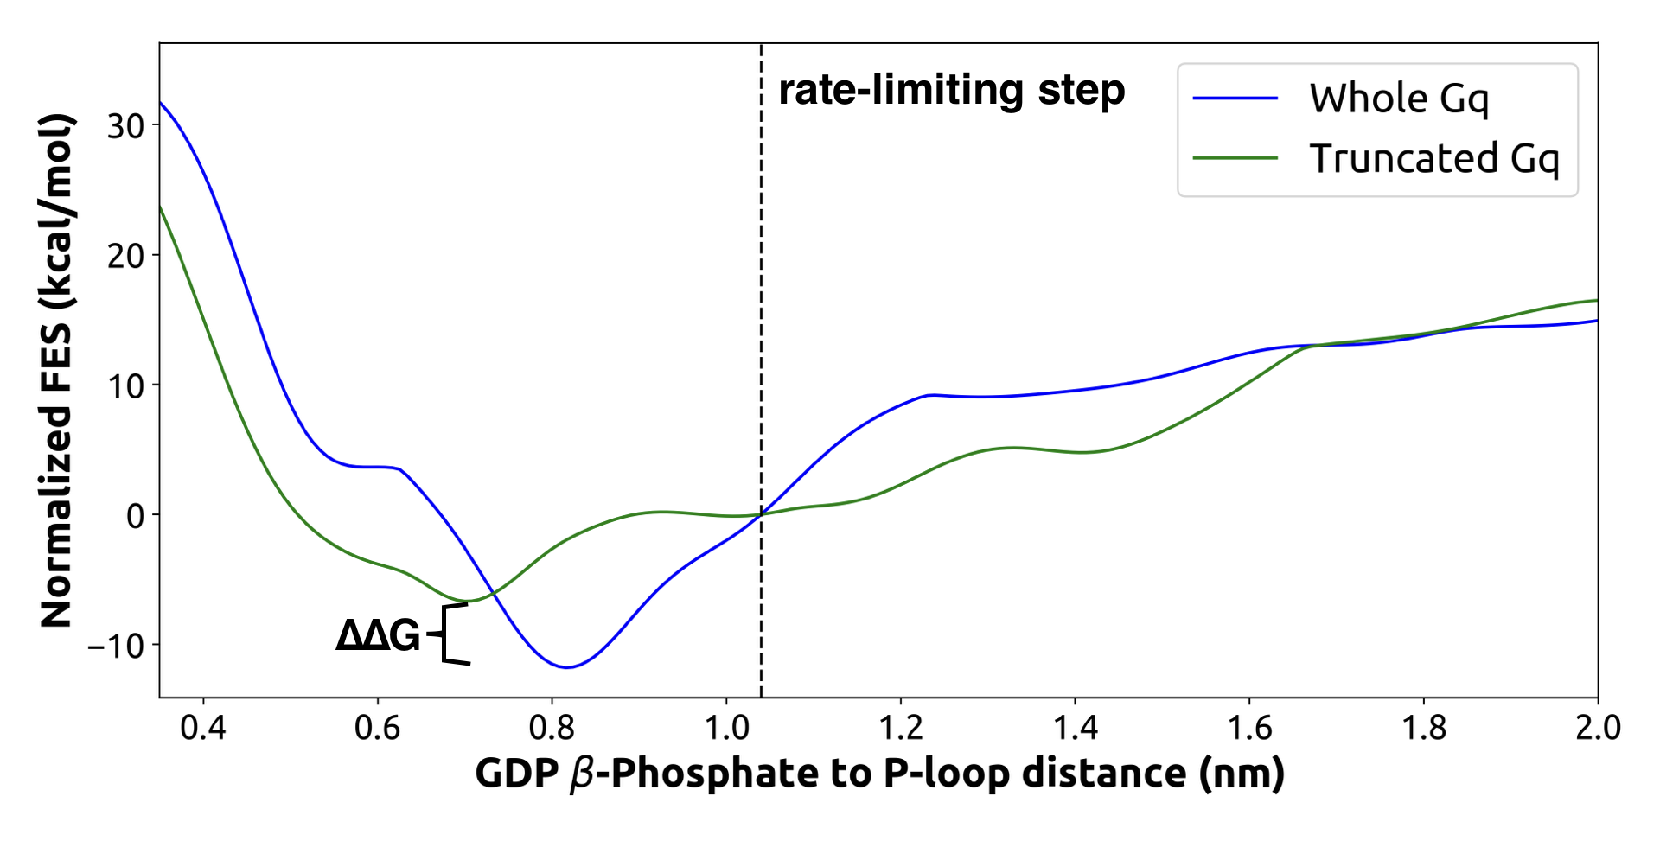
\includegraphics[width=4in]{ch4-fig2-supp1.png}
        \caption[Free-energy surface from metadynamics simulations of GDP release for the full G$\alpha$q (blue) and truncated form (green, without the last five C-terminal residues).]
            {Free-energy surface from metadynamics simulations of GDP release for the full G$\alpha$q (blue) and truncated form (green, without the last five C-terminal residues). Both sets of simulations were run for the same amount of time with identical collective variables. The rate-limiting step as identified from the highest flux pathway is marked with a dashed line. The free-energy difference between the GDP-bound states of the two systems is marked with a bracket.}
        \label{fig:ch4-fig2-supp1}
    \end{figure}

    \begin{figure}[!htb] %Positioning code for figure
        \centering
        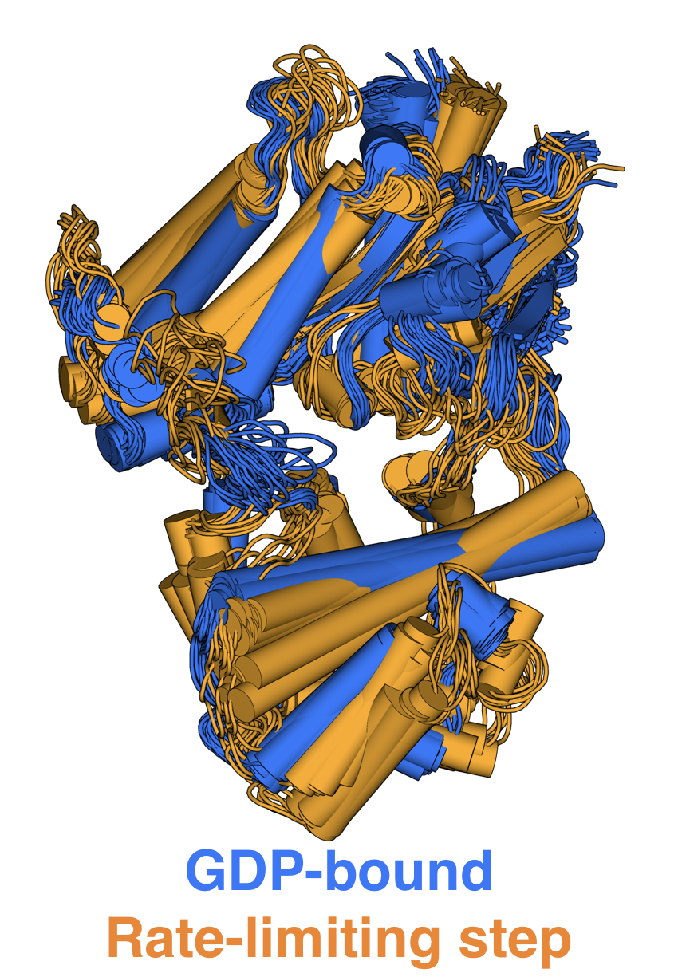
\includegraphics[width=4in]{ch4-fig2-supp2.png}
        \caption[Overlay of representative structures of G$\alpha$q when bound to GDP (blue) or across the rate-limiting step (orange).]
            {Overlay of representative structures of G$\alpha$q when bound to GDP (blue) or across the rate-limiting step (orange).}
        \label{fig:ch4-fig2-supp2}
    \end{figure}

    \begin{figure}[!htb] %Positioning code for figure
        \centering
        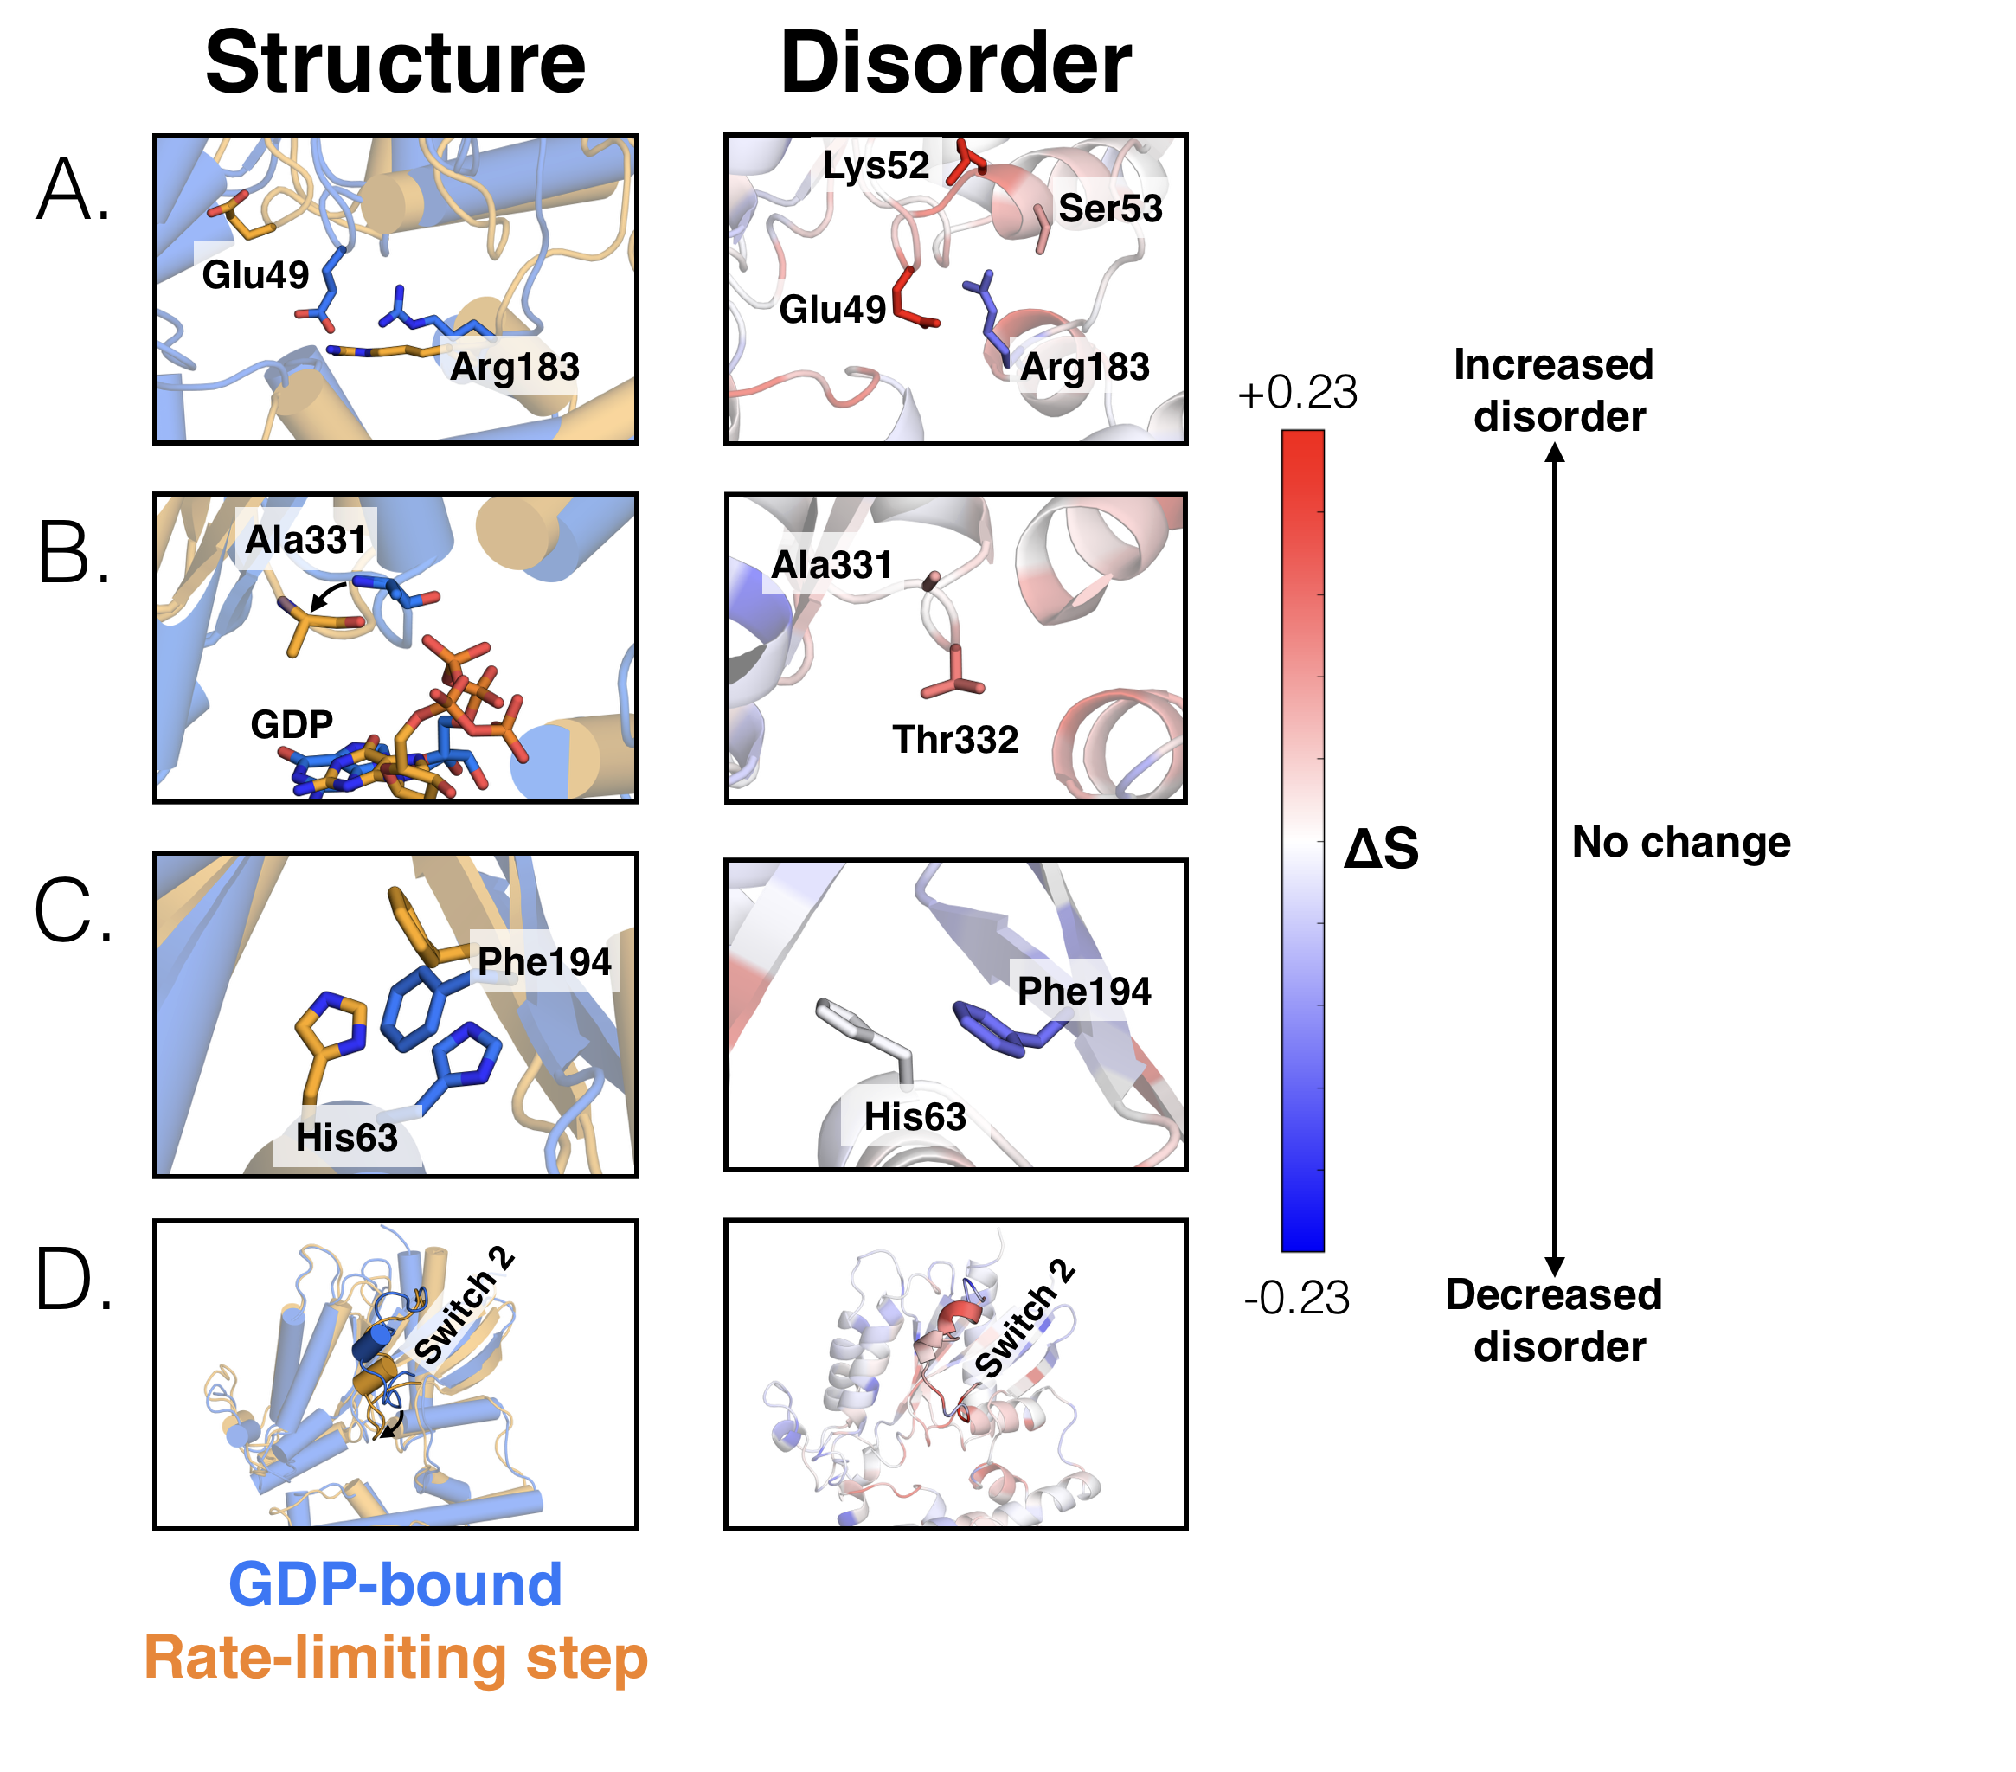
\includegraphics[width=5.5in]{ch4-fig2-supp3.png}
        \caption[Changes in the structure (left) and disorder (right) of specific regions across the rate-limiting step.]
            {Changes in the structure (left) and disorder (right) of specific regions across the rate-limiting step. \textbf{(A)} Residues that contact the phosphates of GDP, including the salt bridge between Glu49$^{G.s1h1.4}$ and Arg183$^{G.hfs2.2}$, \textbf{(B)} the s6h5 loop, \textbf{(C)} the $\pi - \pi$ stacking interaction between Phe194$^{G.S2.6}$ and His63$^{G.H1.12}$, and \textbf{(D)} switch 2.}
        \label{fig:ch4-fig2-supp3}
    \end{figure}

    \begin{figure}[!htb] %Positioning code for figure
        \centering
        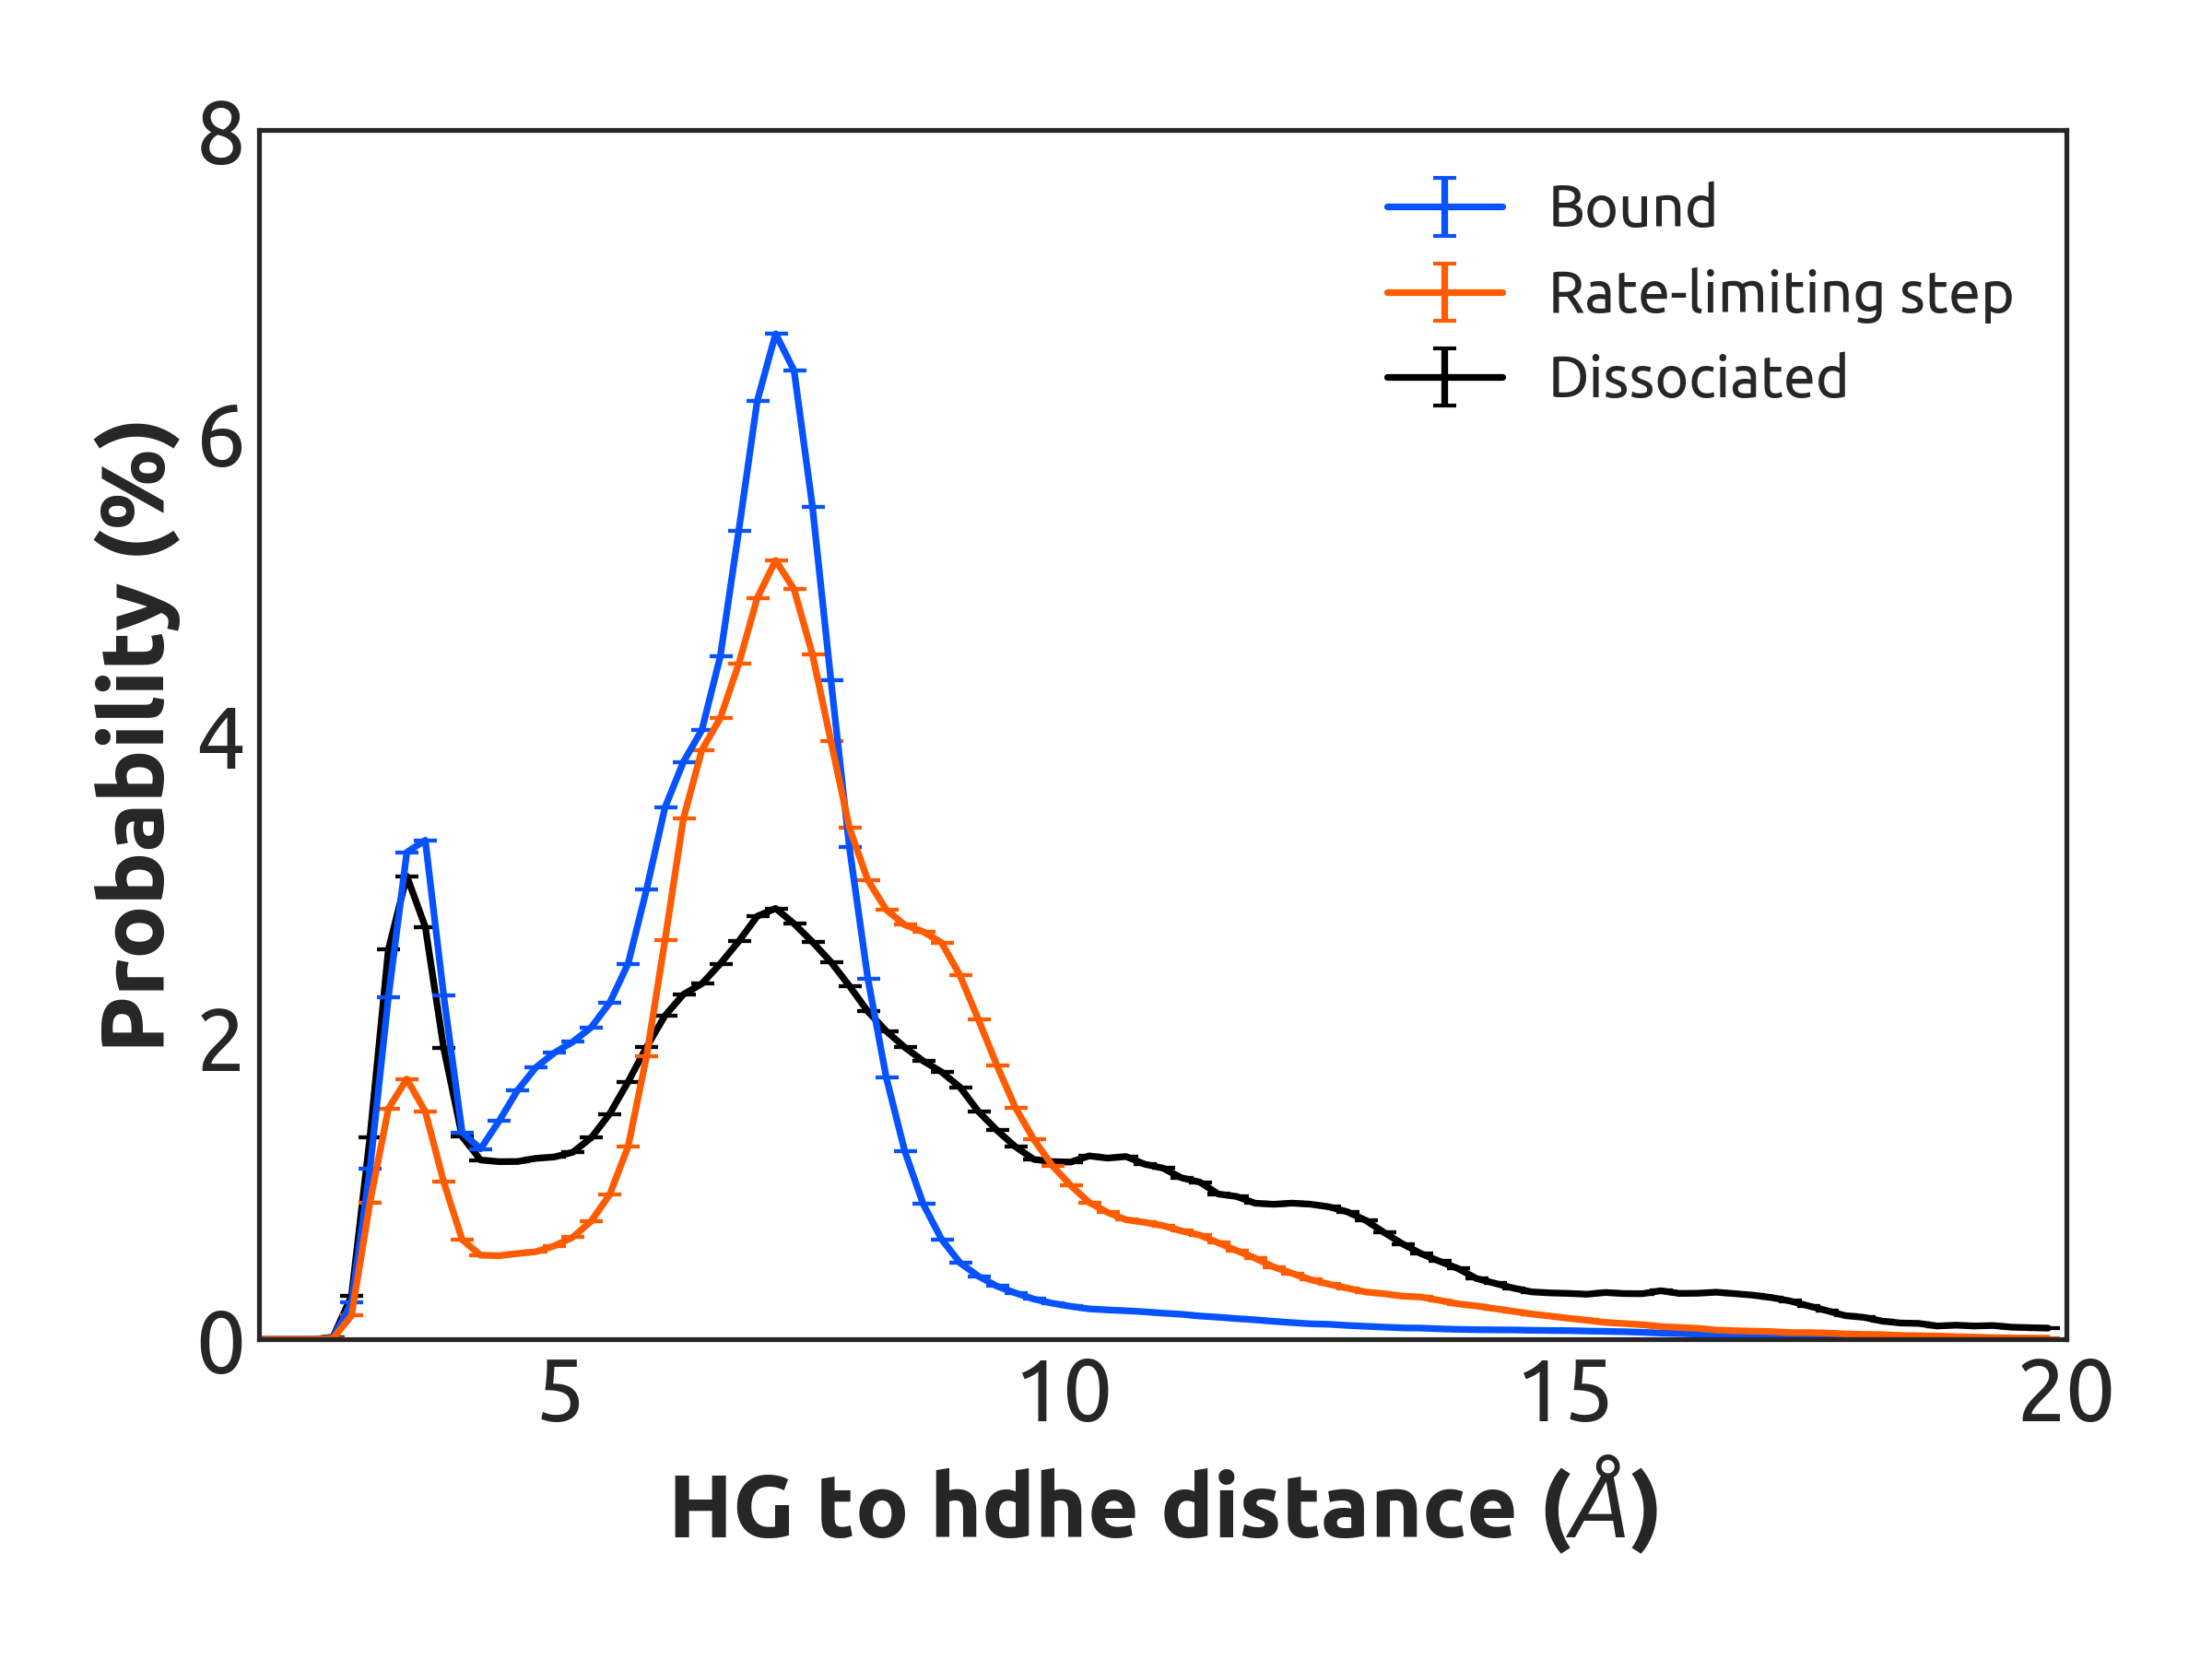
\includegraphics[width=3.5in]{ch4-fig2-supp4.png}
        \caption[Distribution of distances between the side-chains of K275$^{G.s5hg.1}$ and D155$^{H.hdhe.5}$ for the GDP-bound state (blue), across the rate-limiting step (orange), and upon GDP dissociation (black).]
            {Distribution of distances between the side-chains of K275$^{G.s5hg.1}$ and D155$^{H.hdhe.5}$ for the GDP-bound state (blue), across the rate-limiting step (orange), and upon GDP dissociation (black).}
        \label{fig:ch4-fig2-supp4}
    \end{figure}

    \begin{figure}[!htb] %Positioning code for figure
        \centering
        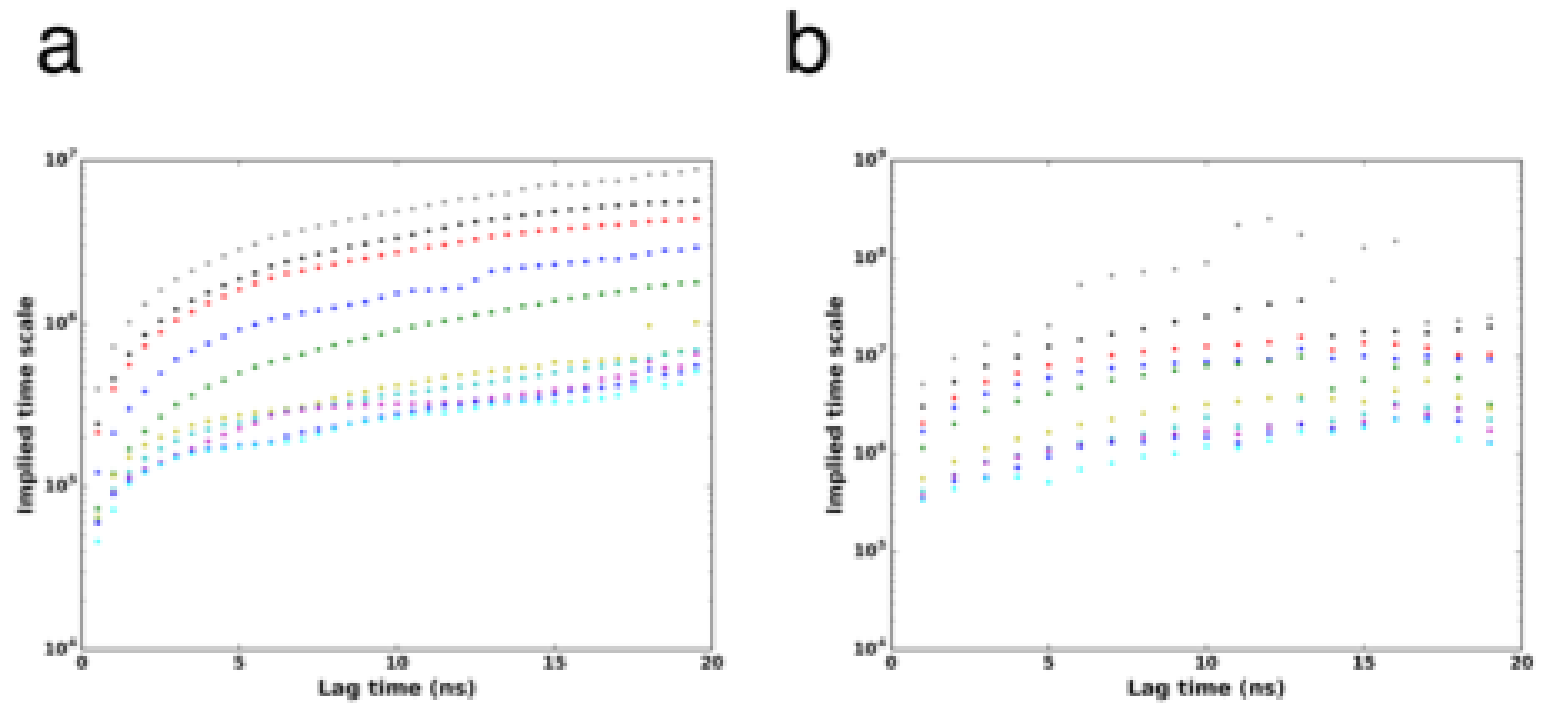
\includegraphics[width=3.16in]{ch4-fig2-supp5.png}
        \caption[Implied timescales for the Markov state model.]
            {Implied timescales for the Markov state model. \textbf{(A)} Top 10 implied timescales for the 5040 states of G$\alpha$. \text{(B)} Top 10 implied timescales for the final 221965 states.}
        \label{fig:ch4-fig2-supp5}
    \end{figure}

    \begin{figure}[!htb] %Positioning code for figure
        \centering
        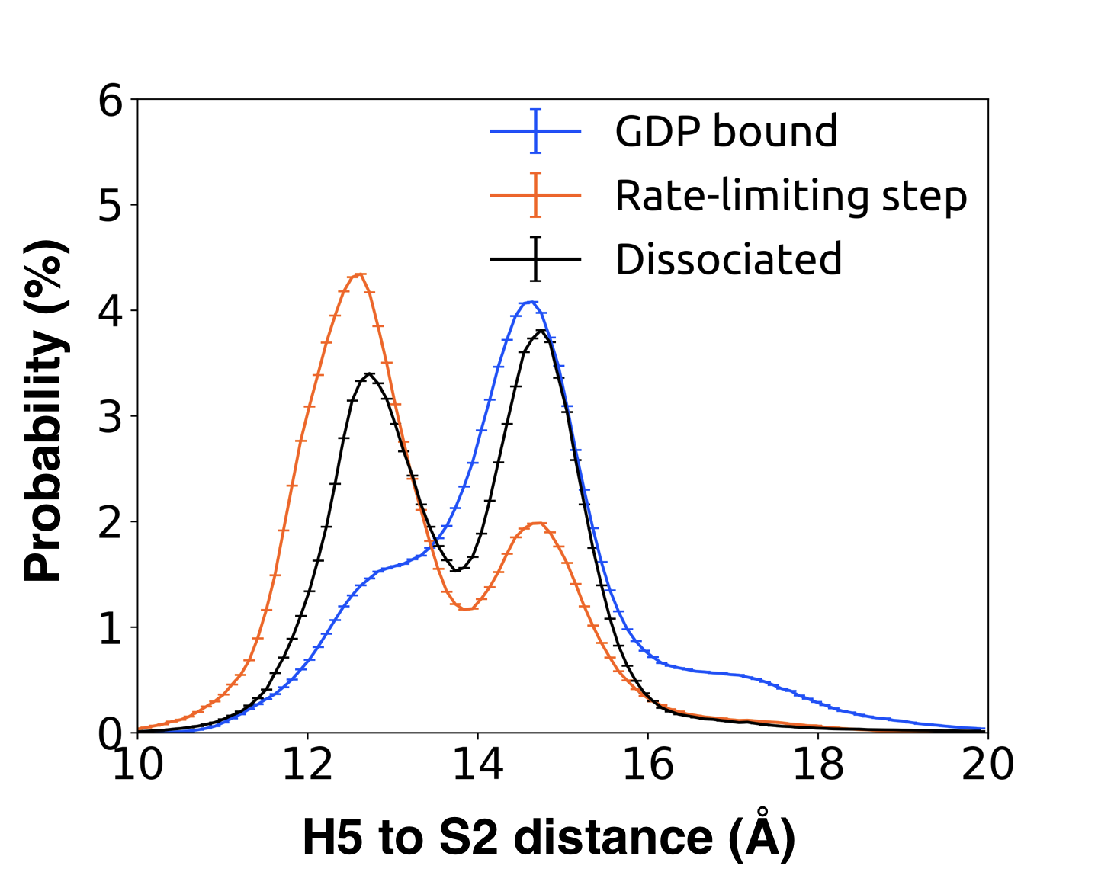
\includegraphics[width=2.5in]{ch4-fig3-supp1.png}
        \caption[Probability distribution of the distance between Leu349$^{G.H5.16}$ on H5 and Phe194$^{G.S2.6}$ on S2 to monitor the tilting motion of H5 upon GDP release when bound to GDP (blue), across the rate-limiting step (orange), and upon GDP dissociation (black).]
            {Probability distribution of the distance between Leu349$^{G.H5.16}$ on H5 and Phe194$^{G.S2.6}$ on S2 to monitor the tilting motion of H5 upon GDP release when bound to GDP (blue), across the rate-limiting step (orange), and upon GDP dissociation (black). In the GDP bound state (blue), such a distance is peaked at 15 \AA. Across the rate-limiting step (orange), tilting motion of H5 upon GDP release occurs with a peak in distance at 12.5 \AA.}
        \label{fig:ch4-fig3-supp1}
    \end{figure}

    \begin{figure}[!htb] %Positioning code for figure
        \centering
        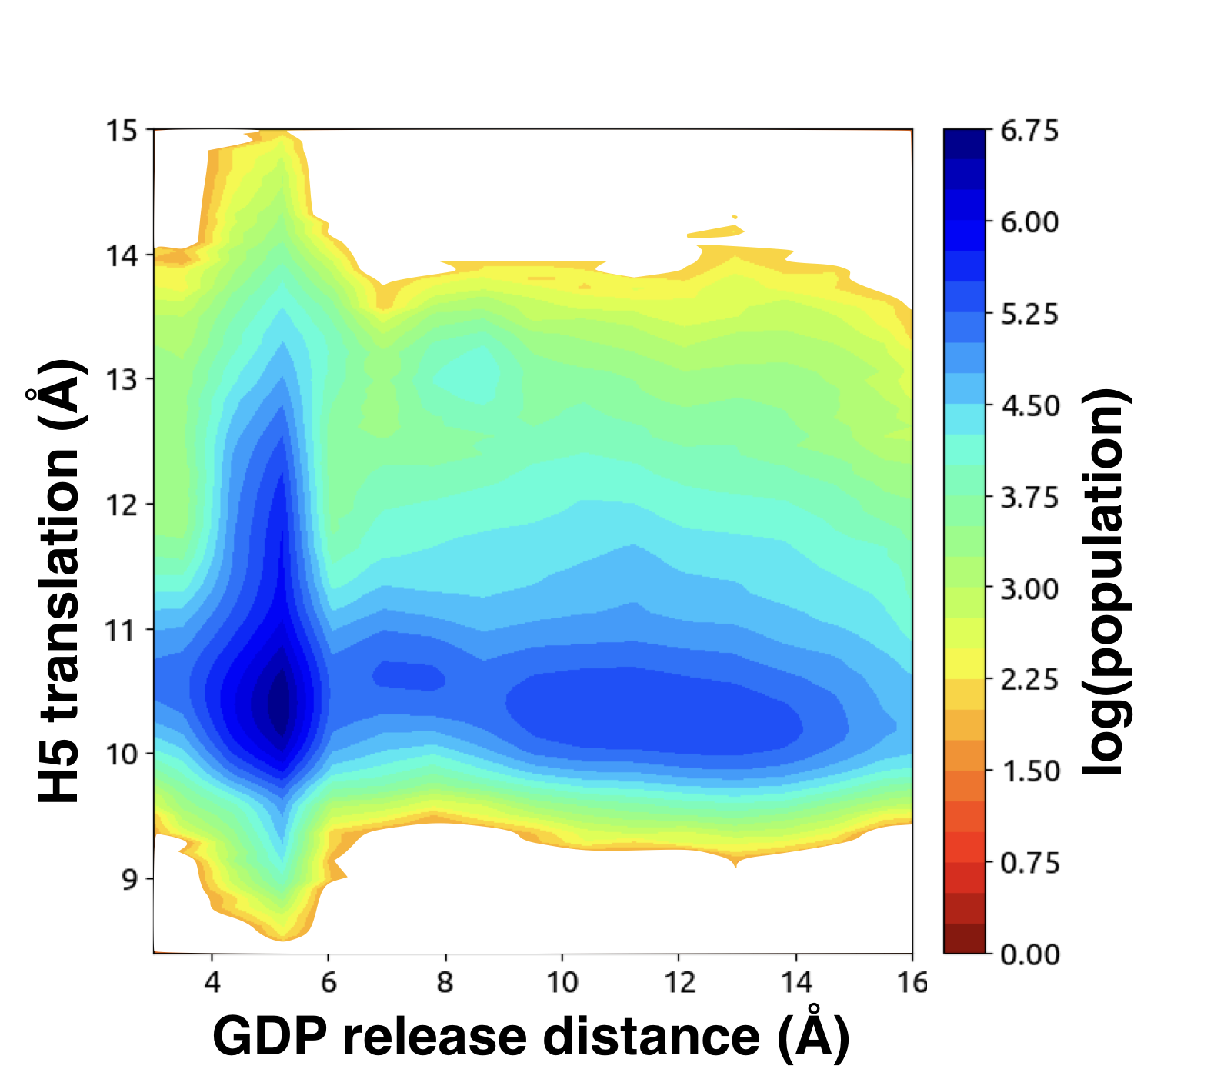
\includegraphics[width=3.16in]{ch4-fig3-supp2.png}
        \caption[H5 vertical motion is sampled across GDP release simulations.]
            {H5 vertical motion is sampled across GDP release simulations. At each point, the combined population (represented by the color scale) of that state is shown using both GDP-bound and intermediate stages of the GDP release pathway. H5 vertical motion was measured by computing the distance between Thr334$^{G.H5.1}$ on the s6h5 loop and Phe341$^{G.H5.8}$ on H5. GDP release distance was measured as the distance from GDP $\beta$-phosphate to the center of mass between residues Lys52$^{G.H1.1}$, Ser53$^{G.H1.2}$, and Thr54$^{G.H1.3}$ on H1.}
        \label{fig:ch4-fig3-supp2}
    \end{figure}


    % \setcounter{table}{1} 
    \begin{table}[]
    \centering
    \caption{Measurements comparing tilting and translation of H5 across PDB structures and MD simulation.}
    \label{tab:galpha-struc-compares}
    \begin{tabular}{|l|l|l|l|l|l|}
    \hline
    Construct description &
      PDB ID &
      \begin{tabular}[c]{@{}l@{}}H5 Tilting \\ Distance (\AA)\end{tabular} &
      \begin{tabular}[c]{@{}l@{}}H5 Vertical \\ translation distance (\AA)\end{tabular} &
      \begin{tabular}[c]{@{}l@{}}H5 Tilting \\ residues used\end{tabular} &
      \begin{tabular}[c]{@{}l@{}}H5 Translation\\  residues used\end{tabular} \\ \hline
    G$\alpha$q-GDP       & 3AH8 & 13.5 & 10.6 & Tyr325 to Leu349 & Thr334 to Phe341 \\ \hline
    {\begin{tabular}[c]{@{}l@{}}G$\alpha$q after rate\\ limiting step from MD\end{tabular}} &
      {N/A} &
      {15.1} &
      {11.1} &
      {Tyr325 to Leu349} &
      {Thr334 to Phe341} \\ \hline

    G$\alpha$i-GDP       & 1GP2 & 10.3 & 10.2 & Tyr320 to Ile343 & Thr329 to Phe336 \\ \hline

    G$\alpha$i-µOR       & 6DDF & 14.6 & 13.0 & Tyr320 to Ile343 & Thr329 to Phe336 \\ \hline

    G$\alpha$i-A1AR      & 6D9H & 13.8 & 10.1 & Tyr321 to Ile344 & Thr330 to Phe327 \\ \hline

    G$\alpha$i-Rhodopsin & 6CMO & 15.8 & 10.7 & Tyr320 to Ile343 & Thr329 to Phe336 \\ \hline

    G$\alpha$o-5HT1B     & 6G79 & 13.1 & 14.2 & Tyr310 to Ile333 & Thr319 to Phe326 \\ \hline

    G$\alpha$s-B2AR      & 3SN6 & 12.8 & 14.6 & Tyr360 to Ile383 & Thr369 to Phe376 \\ \hline
    \end{tabular}
    \end{table}%The table above does not make a link or count in the list of figures, so I had to make a blank table with just the caption.
    % \begin{table*}[!h]
    % \caption{Panther protein class description for proteins in \autoref{tab:4_ProteinExpression}.}
    % \end{table*}

    \begin{figure}[!htb] %Positioning code for figure
        \centering
        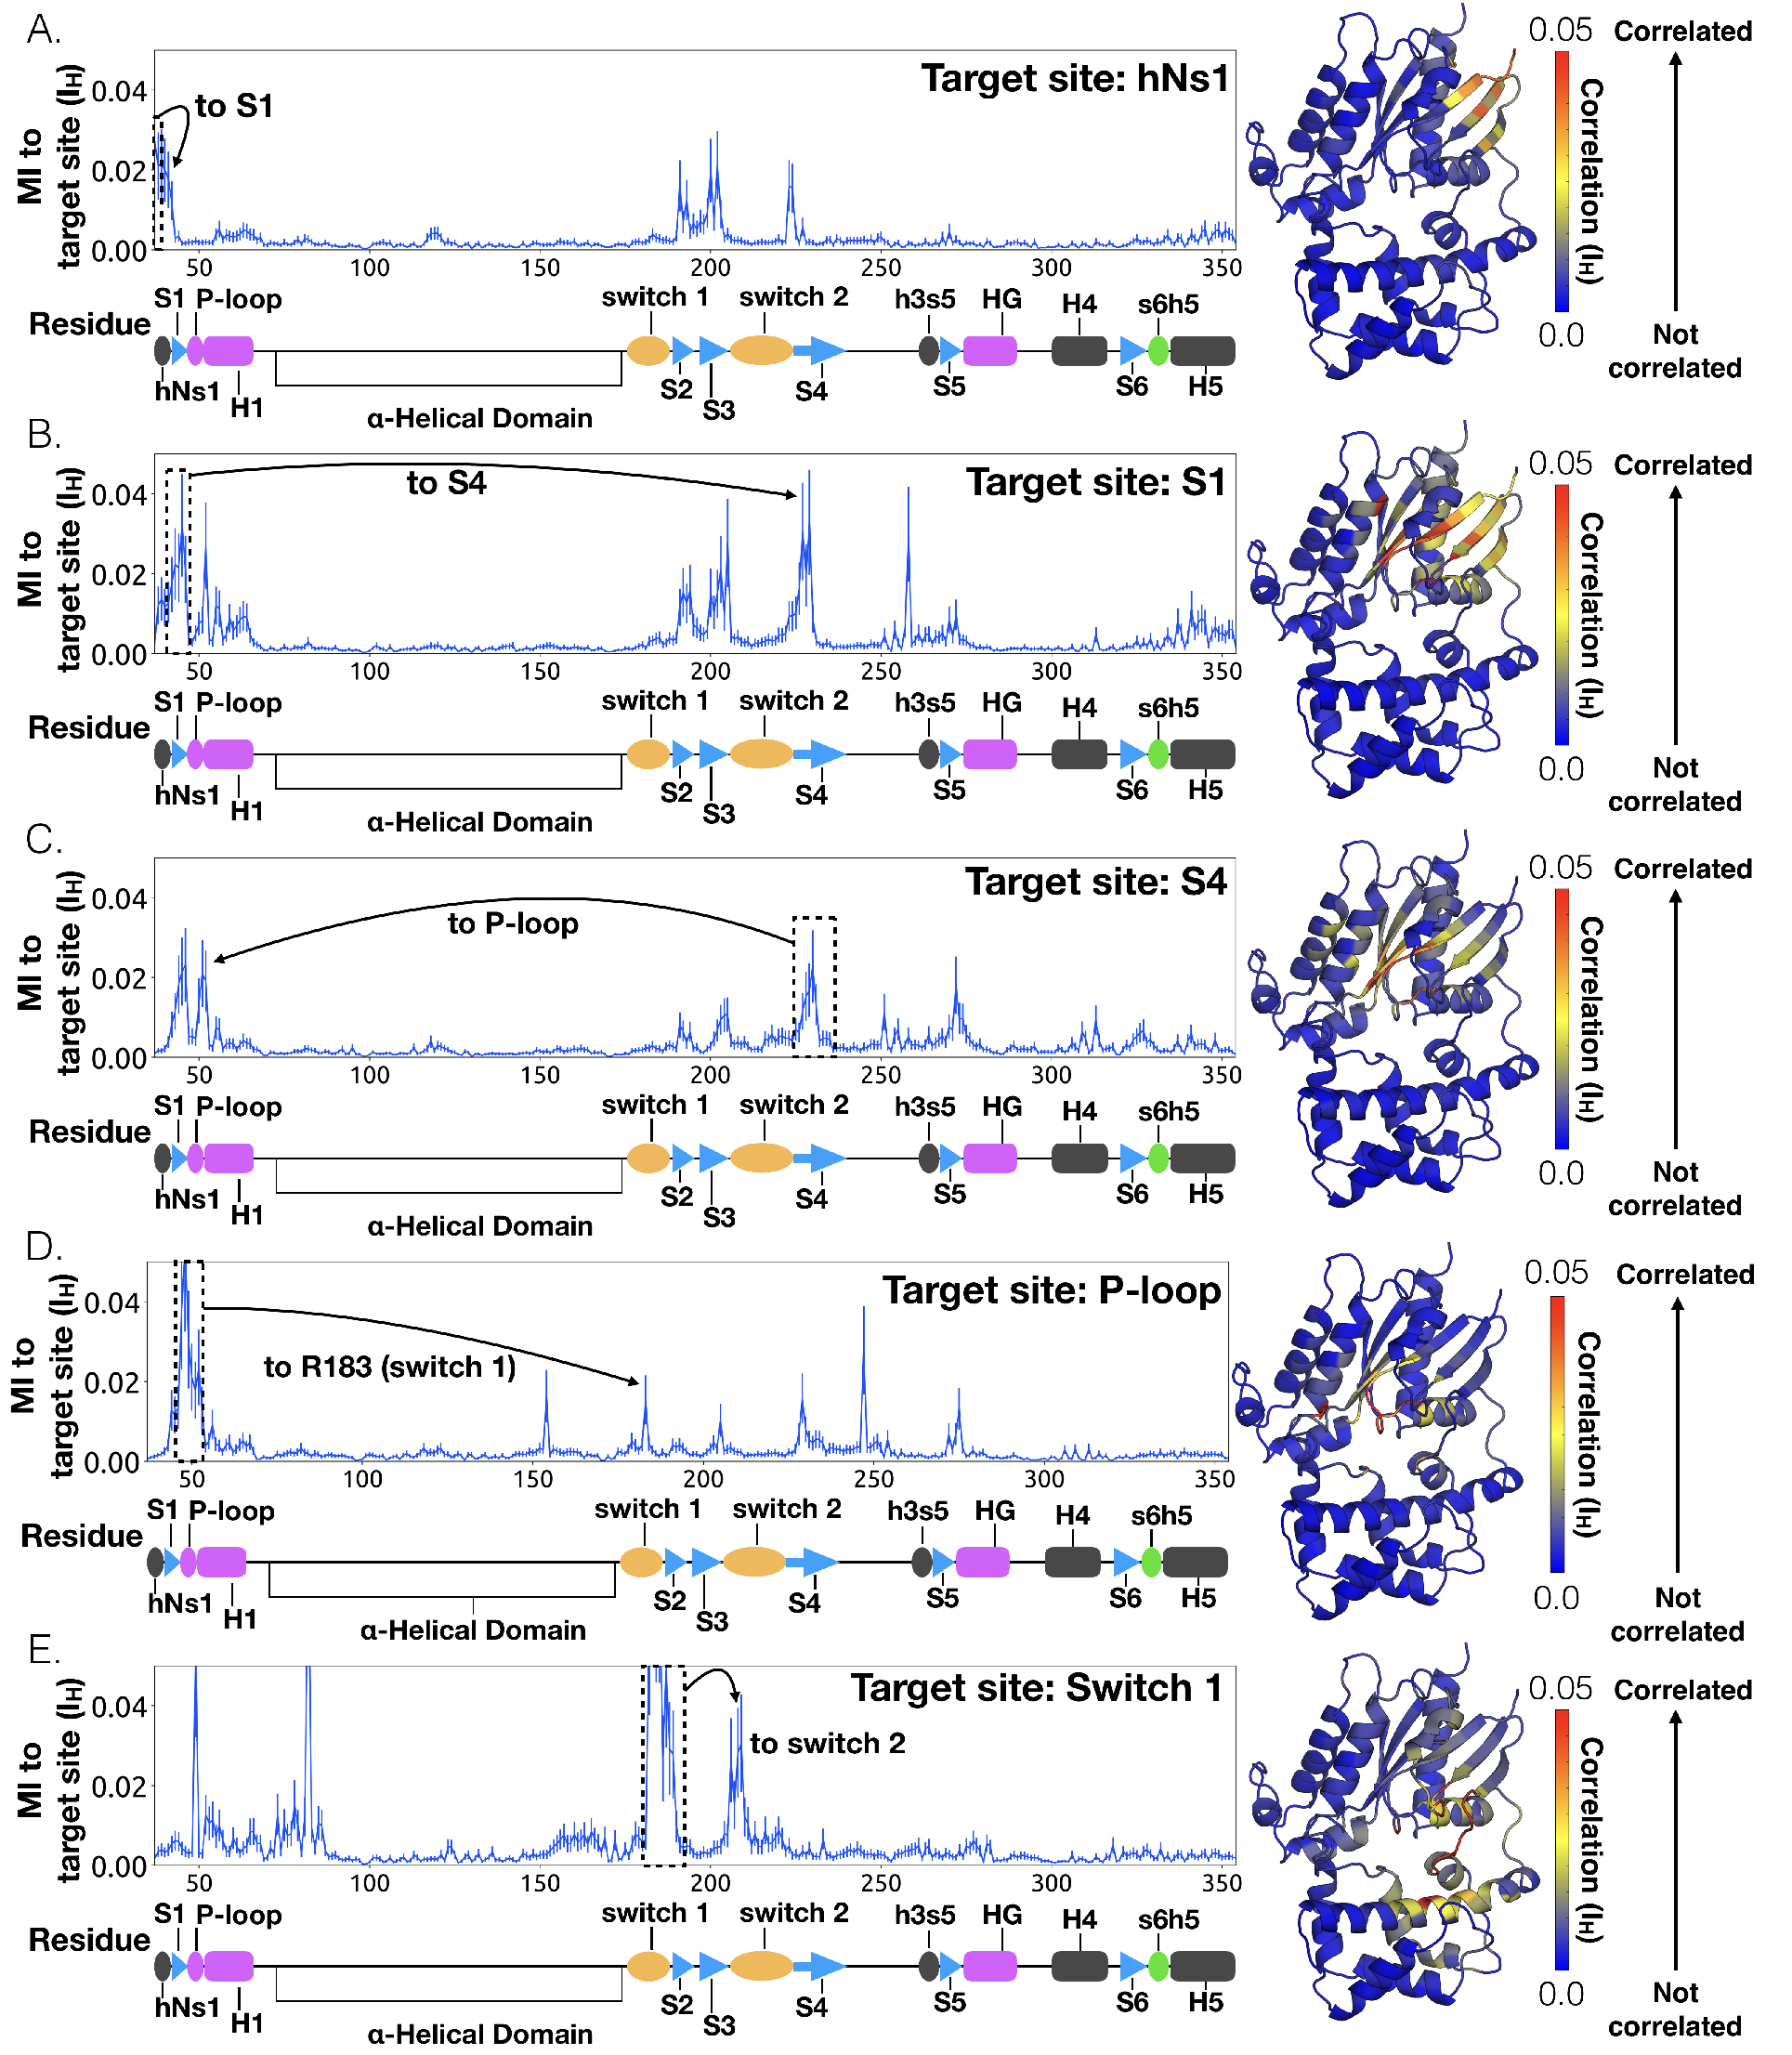
\includegraphics[width=5.6in]{ch4-fig7-supp1.png}
        \caption[Allosteric network connecting hNs1 contacts to the P-loop and switch 1 via S4.]
            {Allosteric network connecting hNs1 contacts to the P-loop and switch 1 via S4. CARDS data showing communication per residue to a target site (dashed box) is plotted (left) and mapped onto the structure of G$\alpha$q (right) for \textbf{(A)} hNs1, \textbf{(B)} S1 \textbf{(C)} S4 \textbf{(D)} the P-loop and \textbf{(E)} Switch 1. Arrows indicate important regions with significant communication to the target site.}
        \label{fig:ch4-fig7-supp1}
    \end{figure}

    \begin{figure}[!htb] %Positioning code for figure
        \centering
        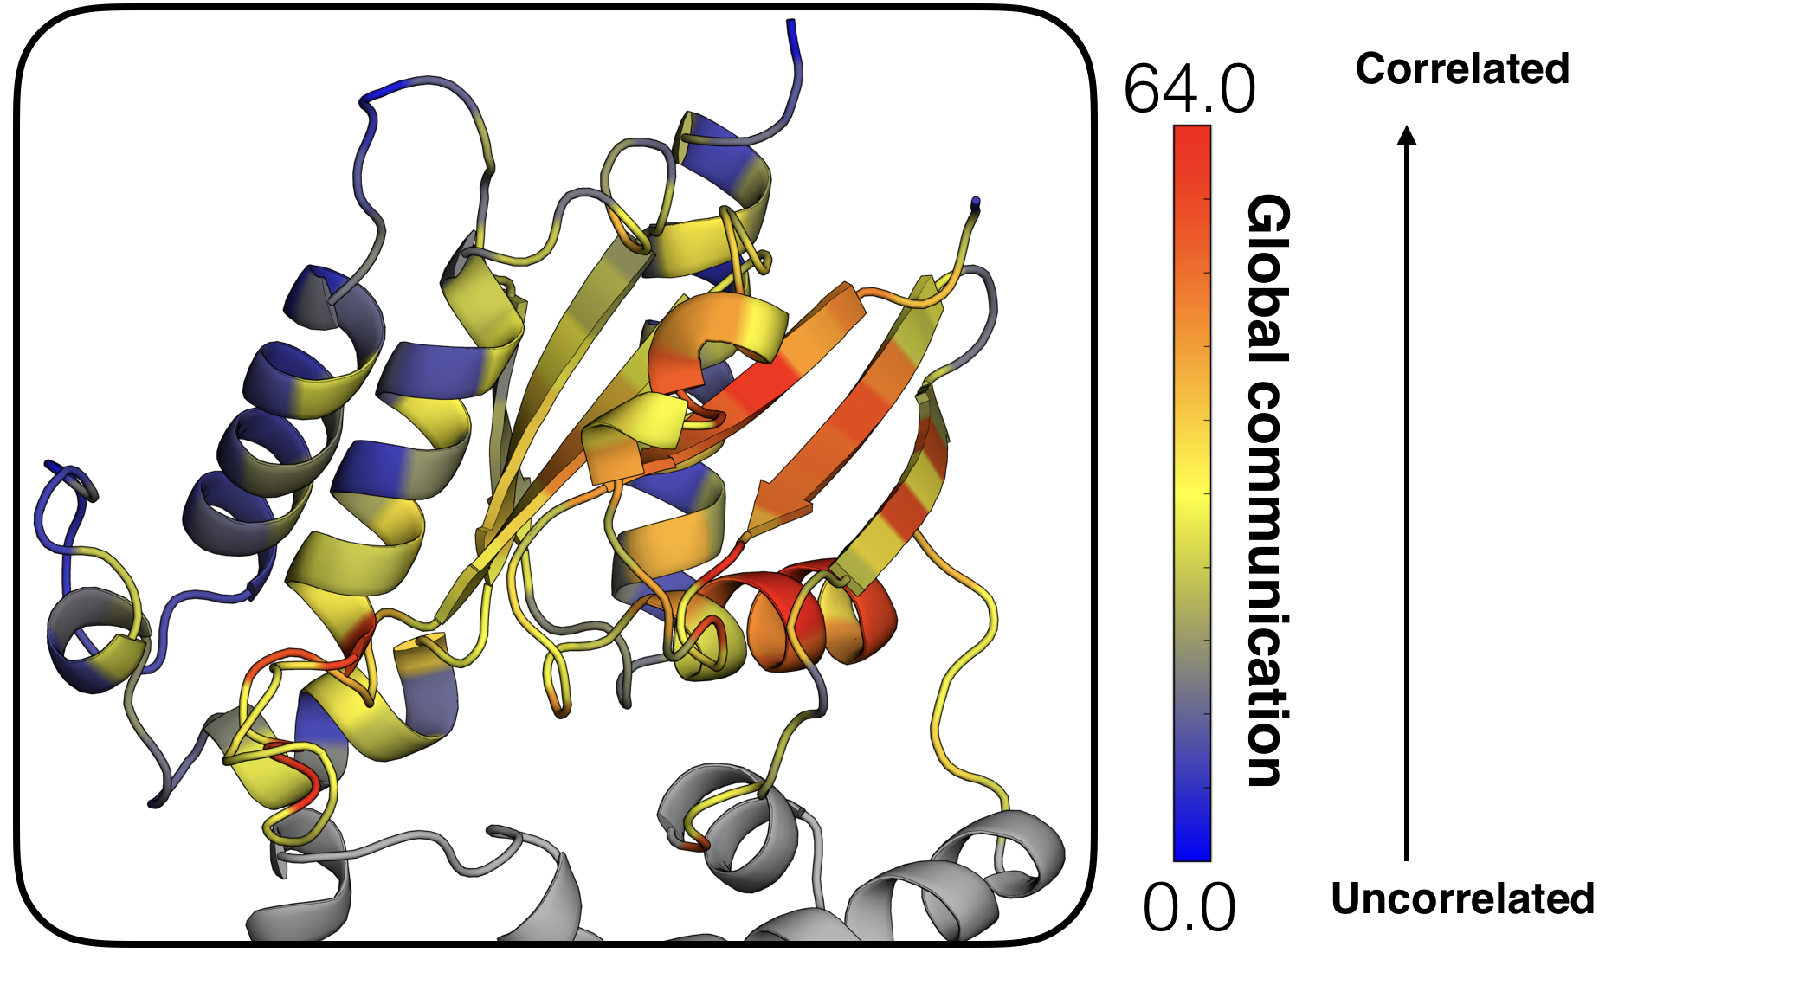
\includegraphics[width=5in]{ch4-fig8-supp1.png}
        \caption[Global communication of each residue in the Ras-like domain mapped onto the structure of G$\alpha$q, colored based on the scale (right). ]
            {Global communication of each residue in the Ras-like domain mapped onto the structure of G$\alpha$q, colored based on the scale (right). The helical domain (gray) is shown for orientation.}
        \label{fig:ch4-fig8-supp1}
    \end{figure}

    \begin{figure}[!htb] %Positioning code for figure
        \centering
        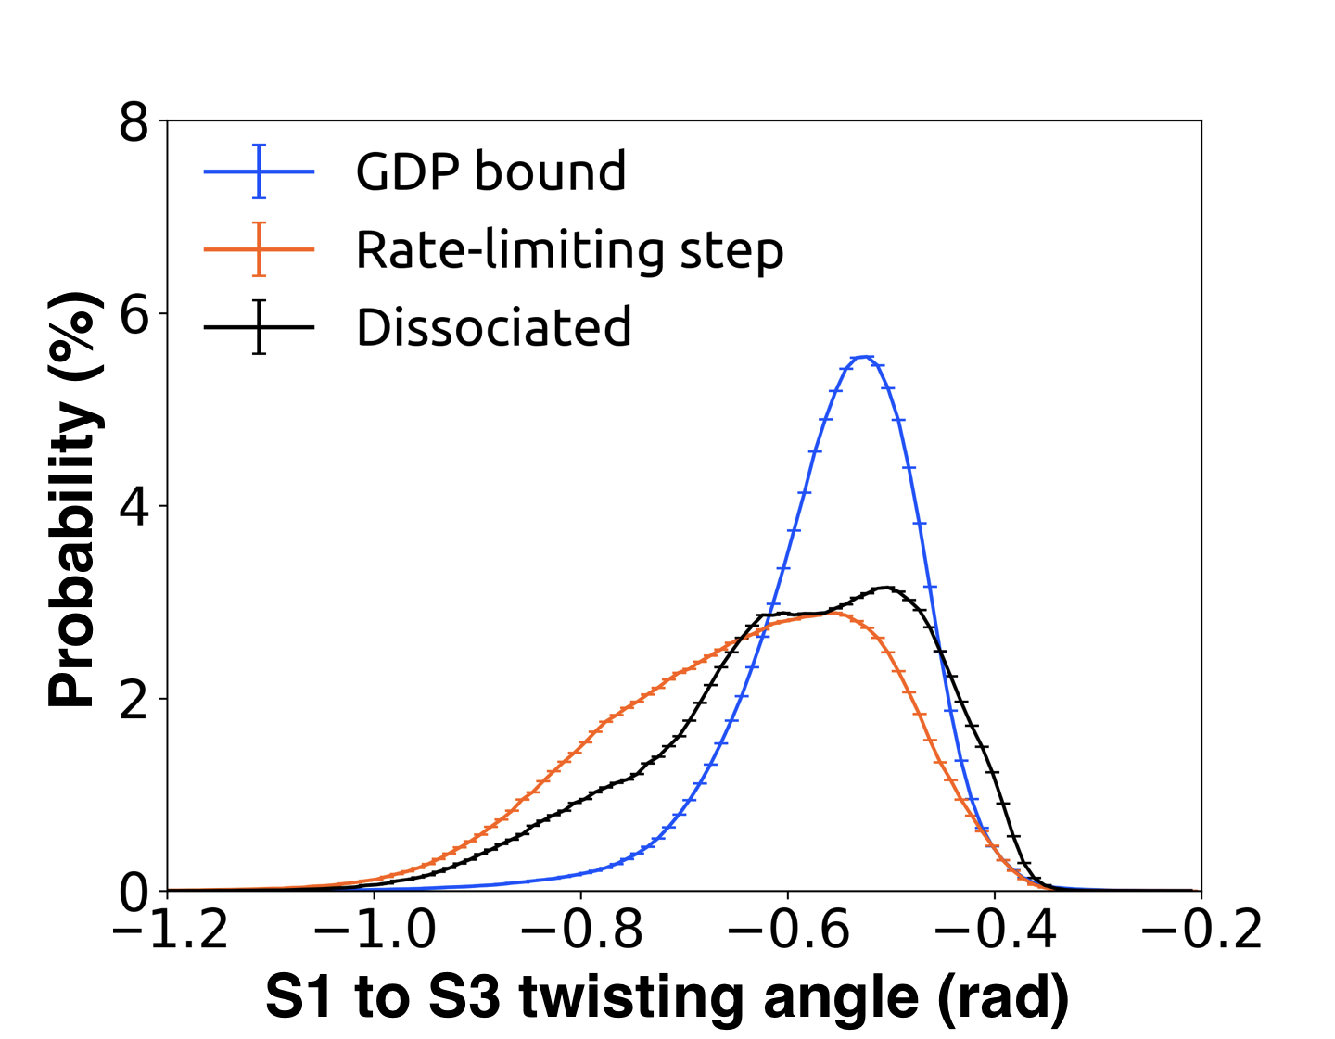
\includegraphics[width=5in]{ch4-fig9-supp1.png}
        \caption[Probability distributions of the twist angle between S1 and S3.]
            {Probability distributions of the twist angle between S1 and S3. The dihedral angle is computed by taking the dihedral angle between the CA atoms of Leu45$^{G.S1.7}$, Leu40$^{G.S1.2}$, Val199$^{G.S3.1}$, and Asp205$^{G.S3.7}$, so that the angle measured represents S1/S3 twisting at the GPCR facing side. Twist was computed for GDP bound(blue), intermediate(orange), and GDP dissociated states(black).}
        \label{fig:ch4-fig9-supp1}
    \end{figure}
	
\end{document}